\chapter{Infraestructura utilizada}
\label{infraestructura}
En este capítulo vamos a profundizar en las tecnologías y herramientas que se han empleado a lo largo de este trabajo. Por un lado se explican los lenguajes de programación (JavaScript, Python y Scratch) y los lenguajes de documentos (HTML5 y JSON) utilizados. Por otro lado, hablaremos de TensorFlowJS, Web Audio API y Teachable Machine, tecnologías que nos ofrecen procesamiento de audio en aplicaciones web. Otras aplicaciones como Blender y A-Frame han sido fundamentales para el  modelado 3D y realidad virtual. Finalmente, hablaremos de la plataforma Kibotics, su estructura y las tecnologías web que la componen.
\section{Lenguajes de programación y de documentos}
\subsection{HTML5}
HTML5 es la última versión de HTML cuyas siglas corresponden a \textit{HyperText Markup Language} es el bloque de construcción más básico de la Web\cite{html}. \textit{HyperText} significa hipertexto, se refiere a enlaces que conectan páginas web entre sí, ya sea dentro de un único sitio web o entre sitios web. 
\textit{Markup} significa marca o etiqueta, ya que todas las páginas web están construidas en base a etiquetas. Con ellas se anota texto, imágenes y otros contenidos para mostrar en un navegador web. El formato HTML5 incluye etiquetas como:  \textless head\textgreater, \textless title\textgreater, \textless body\textgreater, \textless header\textgreater, \textless footer\textgreater, \textless article\textgreater, \textless section\textgreater, \textless p\textgreater, \textless div\textgreater, \textless span\textgreater, \textless img\textgreater, \textless aside\textgreater, \textless audio\textgreater, \textless canvas\textgreater, \textless datalist\textgreater, \textless details\textgreater, \textless embed\textgreater, \textless nav\textgreater, \textless output\textgreater, \textless progress\textgreater, \textless video\textgreater, \textless ul\textgreater, \textless ol\textgreater y \textless li\textgreater, entre otras. En la Figura 3.1(a) podemos ver cómo es el uso de las etiquetas para la creación de una página web y en la Figura 3.1(b) cómo se visualizaría en el navegador.

Hablamos de \textit{Language} porque HTML es un lenguaje, tiene sus normas, tiene su estructura y una serie de convenciones que nos sirven para definir tanto la estructura como el contenido de una web. Esto no quiere decir que sea un lenguaje de programación. HTML no tiene estructuras de lenguaje de programación, como los bucles, las condiciones, las funciones, etcétera. HTML5 es un estándar que sirve para definir la estructura y el contenido de una página Web \cite{html2}. 

\begin{figure}[H]
    \begin{subfigure}[b]{0.5\textwidth}
  \centering
    \includegraphics[width=0.9\textwidth, height=0.5\textwidth]{chapters/images/simplehtmlpage.png}
    \caption{Fuente de la página web}
    \label{fig:f2}
  \end{subfigure}
  \begin{subfigure}[b]{0.5\textwidth}
  \centering
    \includegraphics[width=0.9\textwidth, height=0.5\textwidth]{chapters/images/simplehtml.png}
    \caption{Página web visualización}
    \label{fig:f1}
  \end{subfigure}
  \hfill
  
  \caption{Ejemplo de página web con HTML5}
\end{figure}

Generalmente junto con HTML se utilizan otras dos tecnologías web: CSS para la apariencia/presentación y JavaScript para la funcionalidad/comportamiento de una página web.
\\
\\
Kibotics utiliza plantillas basadas en HTML5 en las páginas web que sirve. En este TFG se va a utilizar HTML5 para modificar y crear las plantillas de las páginas web que mostrarán los nuevos ejercicios que vamos a introducir en la plataforma.

\subsection{JavaScript}
JavaScript es un lenguaje de programación interpretado, no necesita compilar los programas para ejecutarlos, pero sí un intérprete que en nuestro caso es el navegador. JavaScript sigue el estándar ECMAScript que se encarga de regir cómo debe ser interpretado, su operatividad y buen funcionamiento. Este lenguaje posee una sintaxis derivada de C y Java pero no tiene nada que ver con ellos.

Se utiliza principalmente para crear páginas web interactivas, que incorporan efectos como texto que aparece y
desaparece, animaciones, acciones que se activan al pulsar botones y ventanas con
mensajes de aviso al usuario\cite{javascript}.

El código JavaScript se ejecuta en el navegador del cliente y permite que éste interactúe con la página web. En la siguiente Figura 3.2 podemos ver un ejemplo de página web interactiva.\footnote{https://martaquintana.github.io/2018-19-CSAAI-Pong/pong-01.html}

\begin{figure}[H]
  \begin{subfigure}[b]{0.5\textwidth}
  \centering
    \includegraphics[width=1\textwidth, height=0.6\textwidth]{chapters/images/pong.png}
    \caption{Página web visualización}
    \label{fig:f1}
  \end{subfigure}
  \hfill
  \begin{subfigure}[b]{0.5\textwidth}
  \centering
    \includegraphics[width=1\textwidth, height=0.6\textwidth]{chapters/images/codigojs.png}
    \caption{Código JavaScript}
    \label{fig:f2}
  \end{subfigure}
  \caption{Ejemplo de página web interactiva con HTML5, CSS3 y JavaScript }
\end{figure}

En este trabajo JavaScript ha sido una pieza clave para su desarrollo y todos los ejercicios se han creado usando este lenguaje de programación.
 
\subsection{Python y Scratch}

Python es un lenguaje de programación orientado a objetos, es un lenguaje interpretado o de \textit{script}, y al igual que JavaScript necesita un programa intermedio que haga de intérprete. Es un lenguaje fuertemente tipado y multiplataforma. Su filosofía es que el código sea legible y tenga  una sintaxis muy limpia. Sencillo pero potente, lenguaje muy usado en la universidad y en el ámbito laboral \cite{python}.

El servidor de Kibotics está programado en Python (usa la tecnología web Django). Los ejercicios disponibles en la plataforma se pueden resolver también con este lenguaje. Para usar Python las páginas web de los ejercicios contienen el editor ACE. ACE es un editor de código incrustable escrito en JavaScript \cite{aceeditor}. Esto permite al usuario escribir el código de la solución del ejercicio en Python e internamente este código se traduce a JavaScript para el correcto funcionamiento de los ejercicios. 

Como hemos comentado en la introducción, Scratch es un lenguaje de programación visual basado en bloques, creado y mantenido por Lifelong Kindergarten group en el MIT Media Lab. Para usar Scratch en Kibotics se usa Blocky, que es una librería de JavaScript desarrollada por Google. Permite usar en una página web un editor de código visual. Es compatible con Chrome, Firefox, Safari, Opera y otros navegadores. Corresponde a tecnologías del lado cliente y no tiene dependencia con el servidor \cite{blocky}.


Los ejercicios planteados en este TFG están resueltos tanto en Python como en Scratch. Al ser una plataforma para el ámbito educativo estos dos lenguajes son una buena alternativa para empezar a programar porque son lenguajes sencillos y con una curva de aprendizaje muy suave. En la Figura 3.3 podemos ver unos ejemplos de soluciones, la Figura 3.3 a para el Sigue líneas en Python y la Figura 3.3 b para el ejercicio del cuadrado en Scratch.

\begin{figure}[H]
  \begin{subfigure}[b]{1\textwidth}
  \centering
    \includegraphics[width=0.95\textwidth, height=0.4\textwidth]{chapters/images/python.png}
    \caption{Solución en Python}
    \label{fig:f1}
  \end{subfigure}
  \hfill
  \begin{subfigure}[b]{1\textwidth}
  \centering
    \includegraphics[width=0.95\textwidth, height=0.4\textwidth]{chapters/images/scratch2.png}
    \caption{Solución en Scratch}
    \label{fig:f2}
  \end{subfigure}
  \caption{Ejemplo de código en Kibotics }
\end{figure}


\subsection{JSON} JSON, cuyas siglas significan \textit{JavaScript Object Notation}, es un formato de intercambio de datos muy ligero. Para nosotros es fácil de leer y escribir, además la interpretación y generación de ficheros es muy sencilla para las máquinas \cite{json}.

JSON es un formato de datos basado en texto estándar para representar datos estructurados con la sintaxis de objetos de JavaScript. Son archivos de texto plano con codificación UTF8, que son compatibles con todos los sistemas. Se utiliza para transmitir datos en aplicaciones web \cite{json2}. 
Este formato puede ser utilizado independientemente de JavaScript, y muchos entornos de programación poseen la capacidad de leer (convertir; \textit{parsear}) y generar ficheros JSON. En nuestro caso vamos a leer ficheros JSON desde JavaScript.

Un fichero JSON  típicamente está compuesto de dos estructuras: 
\begin{itemize}
    \item \textbf{Una colección de pares de nombre/valor}: En otros lenguajes son conocidos como objeto, registro, estructura, diccionario o lista de claves. 
    Ejemplo objeto: 
    \begin{lstlisting}
    {
        "id" : 7,
        "name" : "Robot",
        "type" : "Drone"
    }
     \end{lstlisting}
    \item \textbf{Una lista ordenada de valores}: En la mayoría de los lenguajes, esto se implementa como arreglos \textit{arrays}, vectores o listas.  
     Ejemplo array:  
     \begin{lstlisting}
        [ "blue", "yellow", "orange" ]
     \end{lstlisting}
\end{itemize}

Estas estructuras son universales en todos los lenguajes de programación, es por esto que  JSON es muy fácil utilizar para un programador. Todos los lenguajes disponen de funciones para interpretar cadenas JSON y convertir datos en cadenas JSON válidas.

En la Figura 3.4 podemos ver una pequeña parte de un fichero de configuración de un ejercicio con JSON en Kibotics. En esta plataforma se utiliza JSON para crear los ejercicios con las características específicas que le correspondan y en este TFG se han usado tanto para la creación de los mundos como para fijar las posiciones de los confetis en el ejercicio del Roomba que veremos más adelante.

\begin{figure}[H]
    \centering
    \includegraphics[width=0.6\textwidth, height=0.4\textwidth]{chapters/images/json.png}
    \caption{Parte de un fichero config.json de un ejercicio en Kibotics}
    \label{fig:my_label}
\end{figure}

\section{Herramientas}
\subsection{TensorFlowJS, Web Audio API y Teachable Machine}
Para procesar el audio en JavaScript se han tenido que analizar diferentes herramientas o APIs\footnote{Interfaz de programación de aplicaciones} de procesamiento de audio en la web. De esta forma hemos podido elegir la herramienta que mejor se adapta a nuestro problema.
Entre ellas TensorFlowJS, Web Audio API y Teachable Machine (Figura 3.5) son las herramientas que se han estudiado para llevar a cabo el teleoperador acústico.
\\
TensorFlowJS es una biblioteca de JavaScript para el entrenamiento y la implementación de modelos de aprendizaje automático en navegadores y en Node.js . TensorFlow es una plataforma de código abierto para la creación de modelos de aprendizaje automático \cite{tfjs}.

La API de Audio Web provee un sistema poderoso y versatil para controlar audio en la Web, permitiendo a los desarrolladores escoger fuentes de audio, agregar efectos al audio, crear visualizaciones de audios y aplicar efectos espaciales, entre otras cosas \cite{waa}.

Teachable Machine es una herramienta basada en la Web que hace posible crear modelos de aprendizaje automático de manera rápida, sencilla y accesible para todos \cite{tm}.

\begin{figure}[H]
    \centering
    \begin{subfigure}{.3\linewidth}
        \includegraphics[width=1\textwidth]{chapters/images/tfjs.png}
        \caption{Tensor Flow JS}
    \end{subfigure}
    \hskip2em
    \begin{subfigure}{.3\linewidth}
    \includegraphics[width=1\textwidth]{chapters/images/waa.png}
        \caption{Web Audio API}
    \end{subfigure}
    \begin{subfigure}{.3\linewidth}
       \includegraphics[width=1\textwidth, height=0.7\textwidth]{chapters/images/tm.png}
        \caption{Teachable Machine}
    \end{subfigure}
    \caption{Herramientas de reconocimiento de audio}
\end{figure}


En el Capítulo 6 se explicará en profundidad cómo se han usado estas tecnologías y por qué después de probar con cada una de estas tres herramientas, hemos elegido Teachable Machine para el desarrollo final del Teleoperador Acústico.


\subsection{A-Frame}

A-Frame es un marco web para crear experiencias de realidad virtual (VR). A-Frame utiliza HTML declarativo, lo que facilita bastante la creación de escenas en 3D y es accesible para todos, desde desarrolladores web, artistas y diseñadores, a educadores y estudiantes. Su estructura entidad-componente proporciona una infinidad de posibilidades y ofrece compatibilidad con \textit{three.js}, una biblioteca  escrita en JavaScript para crear y mostrar gráficos animados 3D en un navegador Web. 

Sin instalar nada, A-Frame permite manejar modelos 3D para crear entornos de realidad virtual solamente usando las etiquetas \textit{\textless script\textgreater  y \textless a-scene\textgreater}. Es compatible con aplicaciones de realidad virtual como GearVR y Windows Mixed Reality entre otras. Además funciona perfectamente en ordenadores y teléfonos inteligentes \cite{aframe}. 


Para crear escenas en una página web solo es necesario importar la librería de A-Frame de la siguiente forma: \begin{lstlisting}
    <script src="https://aframe.io/releases/1.2.0/aframe.min.js"></script>
\end{lstlisting} 
y poner las etiquetas corresponientes a-scene y los objetos que queramos que aparezacan en la escena con sus atributos.
A continuación se muestra un ejemplo de código correspondiente con la visualización de la escena en el navegador en la Figura 3.6.
\\
\begin{lstlisting}
    <html>
      <head>
        <script src="https://aframe.io/releases/1.2.0/aframe.min.js"></script>
      </head>
      <body>
        <a-scene>
          <a-box position="-1 0.5 -3" rotation="0 45 0" color="#4CC3D9"></a-box>
          <a-sphere position="0 1.25 -5" radius="1.25" color="#EF2D5E"></a-sphere>
          <a-cylinder position="1 0.75 -3" radius="0.5" height="1.5" color="#FFC65D"></a-cylinder>
          <a-plane position="0 0 -4" rotation="-90 0 0" width="4" height="4" color="#7BC8A4"></a-plane>
          <a-sky color="#ECECEC"></a-sky>
        </a-scene>
      </body>
    </html>
\end{lstlisting}

\begin{figure}[H]
    \centering
    \includegraphics[width=1\textwidth, height=0.5\textwidth]{chapters/images/aframe.png}
    \caption{Ejemplo escena en A-Frame}
    \label{fig:my_label}
\end{figure}

A-Frame proporciona un inspector visual 3D incorporado (Figura 3.7). Presionando ctrl + alt + i, podemos inspeccionar la escena, esto es muy útil cuando necesitas la posición concreta de un objeto.

\begin{figure}[H]
    \centering
    \includegraphics[width=0.8\textwidth, height=0.5\textwidth]{chapters/images/inspectoraframe.png}
    \caption{Inspector en A-Frame}
    \label{fig:my_label}
\end{figure}


En nuestro caso \textit{a-entity} serán los modelos 3D de los robots que se crearán con Blender  y se usarán componentes como \textit{a-box}, \textit{a-plane}, \textit{a-cylinder} y \textit{a-sphere} para crear componentes adicionales a la escena dándoles sus respectivas texturas. En este trabajo se ha usado la versión 1.1.0 de A-Frame.

\subsection{Blender}
Blender es un software de creación de modelos 3D gratuito, de código abierto y multiplataforma. Este programa se utiliza para el modelado, montaje, animación, simulación y renderizado 3D, así como para la  composición y seguimiento de movimiento, edición de vídeo y animación 2D
\cite{blender}. En este trabajo se ha usado la versión 2.93.0 de Blender.

Para exportar los modelos de Blender se ha usado el formato glTF \textit{(GL Transmission Format)}. Es un formato de archivo para escenas y modelos 3D basado en JSON. De esta forma se pueden integrar los modelos en A-Frame de forma sencilla y rápida.

Este programa se ha utilizado en este proyecto para crear los nuevos robots, escenarios e introducir animaciones a la plataforma. En la Figura 3.8 se muestra un ejemplo de un cubo animado con Blender. 

\begin{figure}[H]
    \centering
    \includegraphics[width=0.7\textwidth, height=0.4\textwidth]{chapters/images/blender.png}
    \caption{Blender}
    \label{fig:my_label}
\end{figure}

\subsection{Plataforma Kibotics}

Kibotics es una plataforma web para docencia en robótica y programación. Esta plataforma se basa en tecnologías web como Django, para la parte servidor. Utiliza un simulador llamado Websim que se apoya en A-Frame para representar los escenarios de los ejercicios en el navegador del usuario.

Esta plataforma en línea ofrece contenidos educativos para facilitar el aprendizaje en programación a alumnos de primaria, secundaria y bachillerato. Ofrece cursos en los lenguajes Scratch y Python. Los ejercicios están disponibles tanto para robots físicos como simulados. Destacan Mbot, Dron Tello y Pibot entre otros.

La simulación de robots reales permite depurar el software al máximo antes de ejecutarlo en un robot físico y así reducir los costes, ya que no necesitas tener un robot para cada alumno y evitar  posibles daños de los robots y accidentes.

Para usar esta plataforma no es necesario instalar nada, solo tener acceso a Internet. Al ser una aplicación web tenemos la ventaja de que es multiplataforma y podemos usarla en distintos dispositivos.

Kibotics tiene la filosofía \textit{Learn by doing}, aprender haciendo. Las lecciones de teoría junto ejercicios prácticos hacen que los contenidos educativos se vayan adaptando según la complejidad de cada ejercicio. En la Figura 3.9 podemos ver algunos de los ejercicios que ofrecen.

\begin{figure}[H]
\begin{subfigure}{.5\textwidth}
  \centering
  % include first image
  \includegraphics[width=.95\linewidth]{chapters/images/chocagira.png}  
  \caption{Choca-gira US}
  \label{fig:sub-first}
\end{subfigure}
\begin{subfigure}{.5\textwidth}
  \centering
  % include second image
  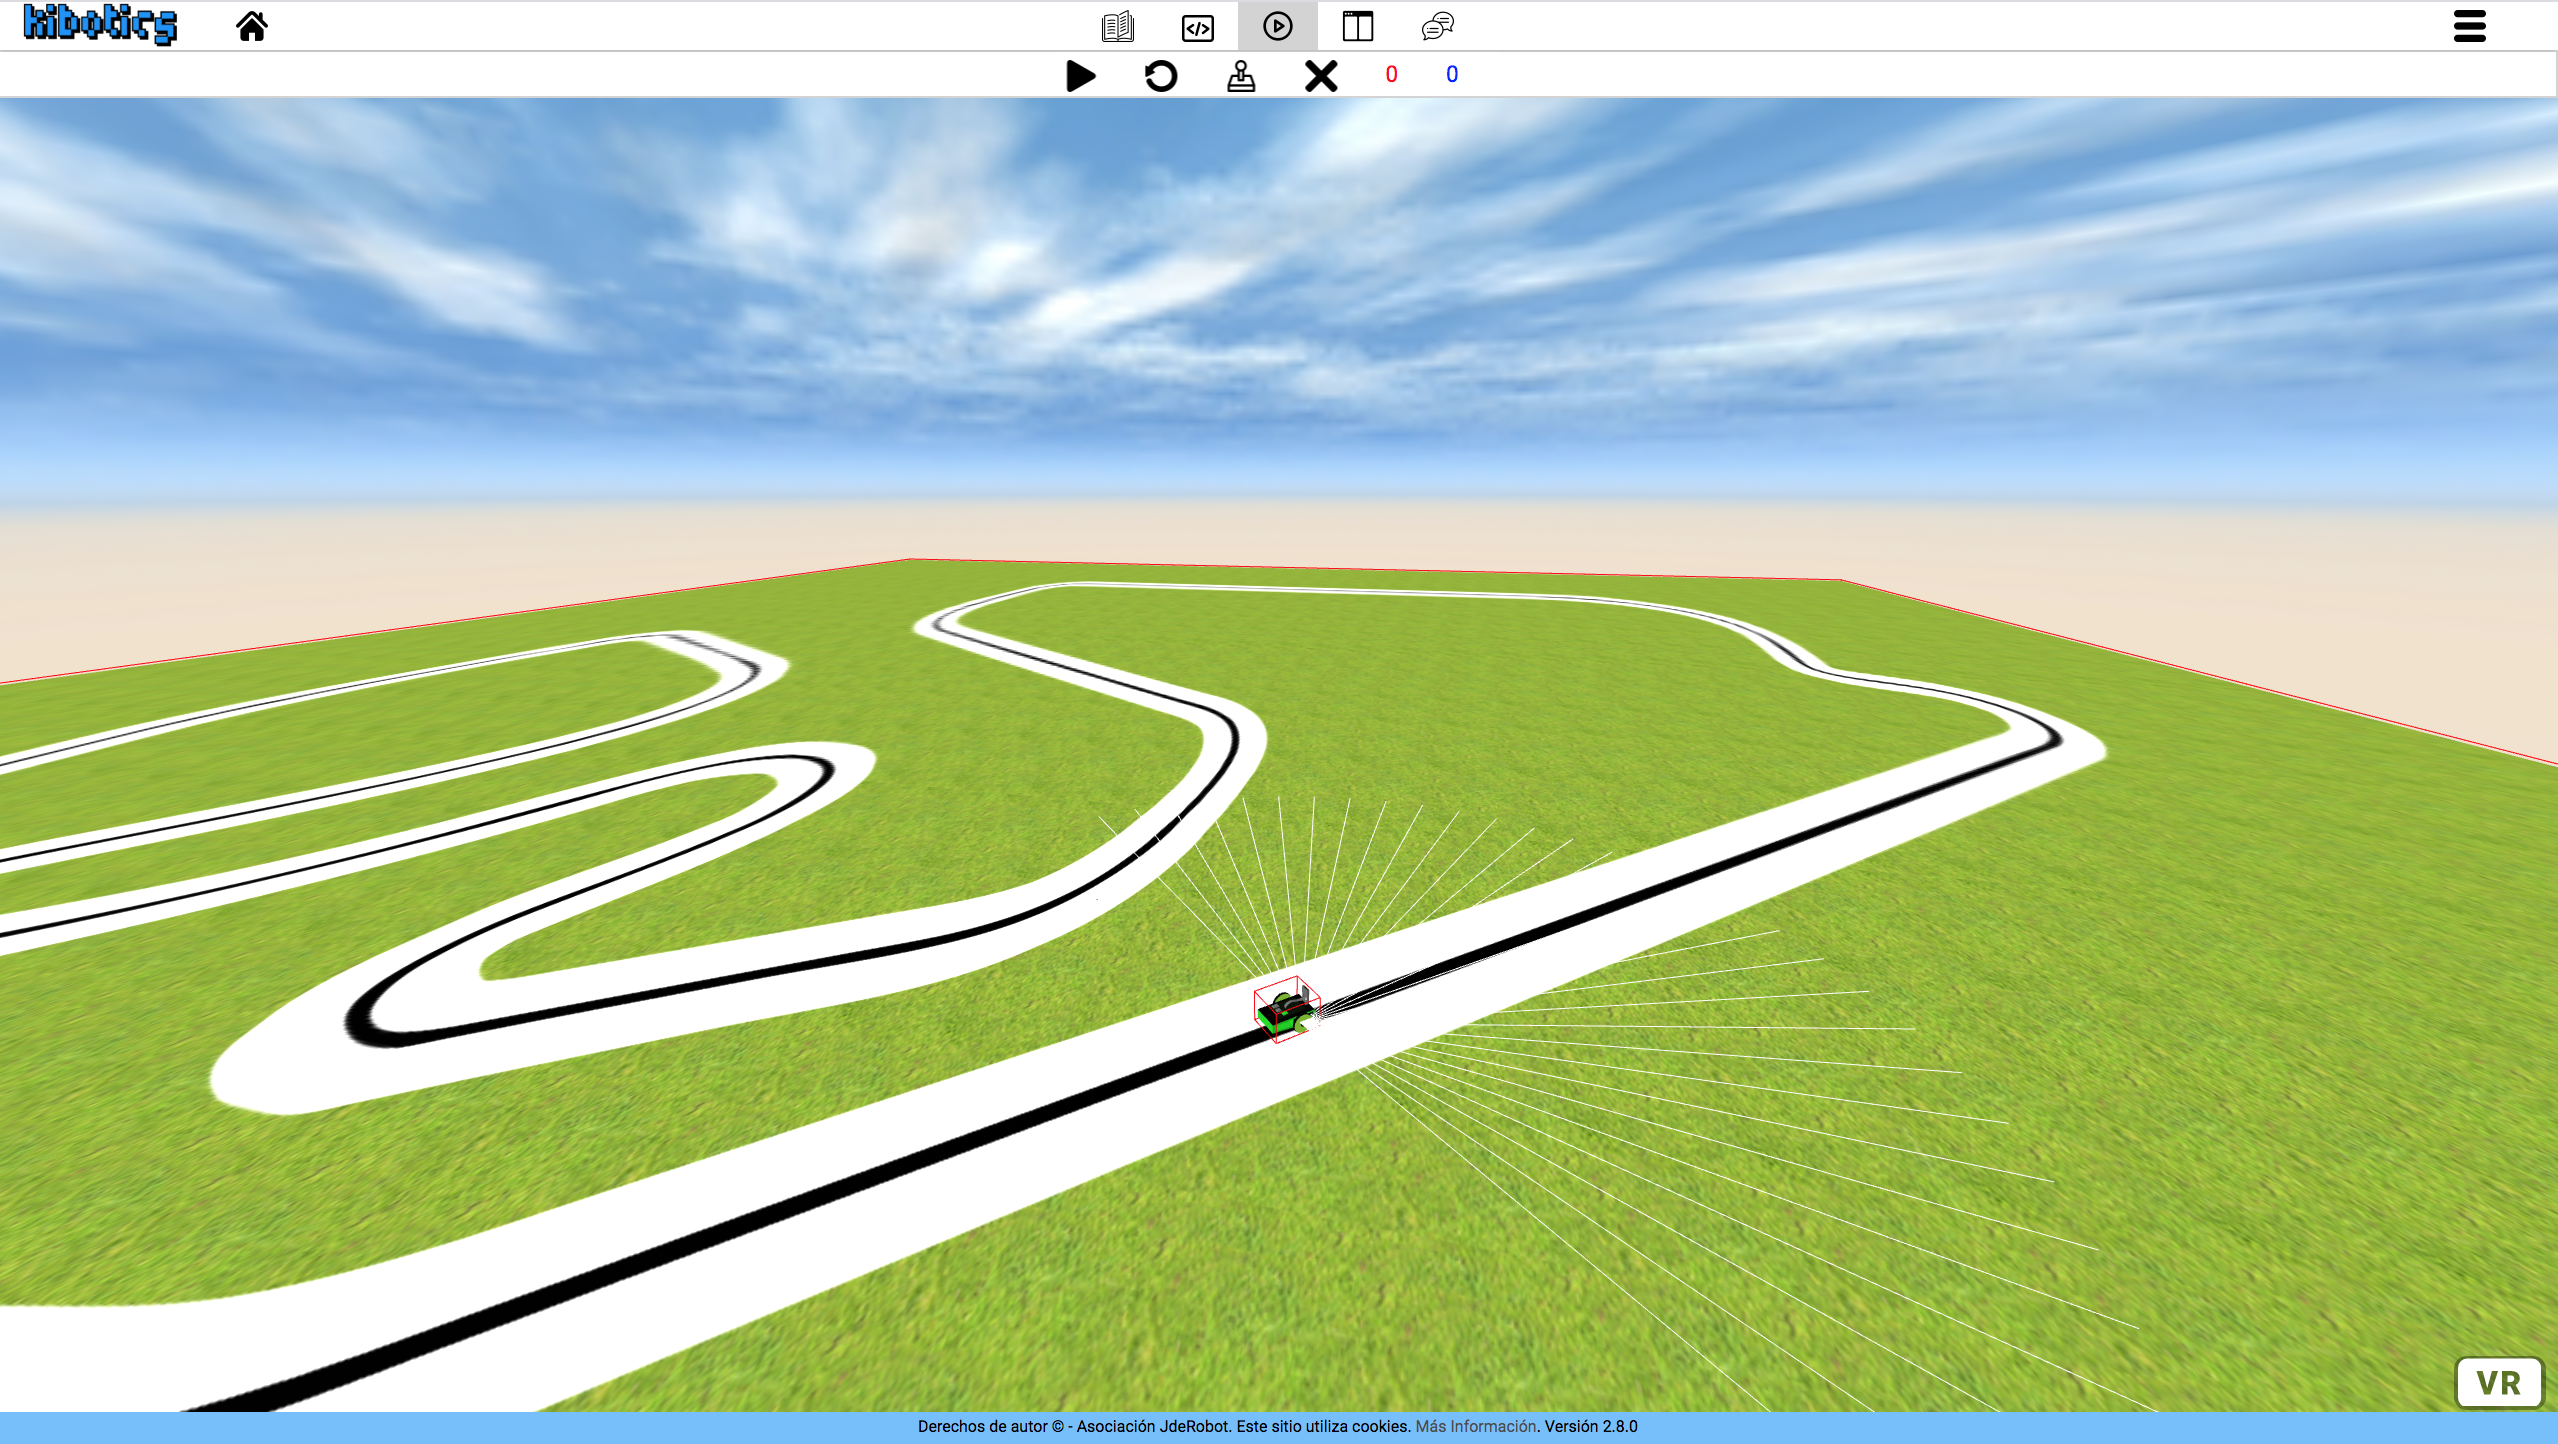
\includegraphics[width=.95\linewidth]{chapters/images/siguelineasir.png}  
  \caption{Sigue líneas IR}
  \label{fig:sub-second}
\end{subfigure}
\begin{subfigure}{.5\textwidth}
  \centering
  % include third image
  \includegraphics[width=.95\linewidth]{chapters/images/atraviesabosque.png}  
  \caption{Atraviesa Bosque}
  \label{fig:sub-third}
\end{subfigure}
\begin{subfigure}{.5\textwidth}
  \centering
  % include fourth image
  \includegraphics[width=.95\linewidth]{chapters/images/colores.png}  
  \caption{Sigue objeto con visión}
  \label{fig:sub-fourth}
\end{subfigure}
\caption{Ejercicios Kibotics}
\label{fig:partes robot}
\end{figure}

Como hemos mencionado anteriormente, la aplicación web Kibotics utiliza la tecnología Django para su servidor. Todos los ejercicios usan la misma plantilla. De esa forma, las páginas se crean dinámicamente con variables de Python y cada ejercicio tiene una página de web diferente con la teoría, el escenario y robot correspondiente.  En estas plantillas o \textit{templates} se incrusta el simulador Websim.

Los robots en Kibotics tienen dos partes: cuerpo y cerebro. El cuerpo se crea con Websim que analiza un fichero JSON (fichero de configuración) y lo materializa gracias a A-Frame. El cerebro lo programa el usuario en su editor en Python o Scratch, donde están implementados los sensores y actuadores gracias a HALRobotAPI. HALRobotAPI\footnote{HAL: Hardware Abstraction Layer} es una capa de abstracción hardware  en la interfaz de programación del robot, ésta proporciona funciones sencillas para manejar los sensores y actuadores del robot . Al ejecutar el ejercicio, dando al botón play que aparece en la página web, el código del cerebro se envía al servidor por Websockets, lo traduce a JavaScript y renderiza el mundo. En la Figura 3.10 podemos ver cómo es la arquitectura de esta aplicación desde una visión general. 

\begin{figure}[H]
    \centering
    \includegraphics[width=1\textwidth, height=0.5\textwidth]{chapters/images/kibotics_arq.png}
    \caption{Arquitectura de la aplicación web Kibotics}
    \label{fig:my_label}
\end{figure}

Kibotics en los últimos años ha ofrecido cursos para la escuela de pensamiento computacional INTEF, el ayuntamiento de Fuenlabrada, la empresa Logix5, Universidad Rey Juan Carlos, IES Martinez Uribarri (Salamanca) y la Comunidad de Madrid \cite{kiboticspdf}.


\subsection{Navegadores web utilizados}

En este Trabajo Fin de Grado se han usado los navegadores Chrome y Firefox por ser los navegadores más extendidos y que proporcionan gran rendimiento, estabilidad y seguridad. Se han utilizado para la visualización de la página web de Kibotics y la ejecución y pruebas de los distintos ejercicios. 
